% Top-level block diagram of the GCD system (task2/gcd_top.vhd, architecture fsmd_io)
% Compile standalone with: pdflatex gcd_top_block_diagram.tex
\documentclass[tikz,border=5mm]{standalone}
\usetikzlibrary{arrows.meta,positioning,calc,fit}

\begin{document}
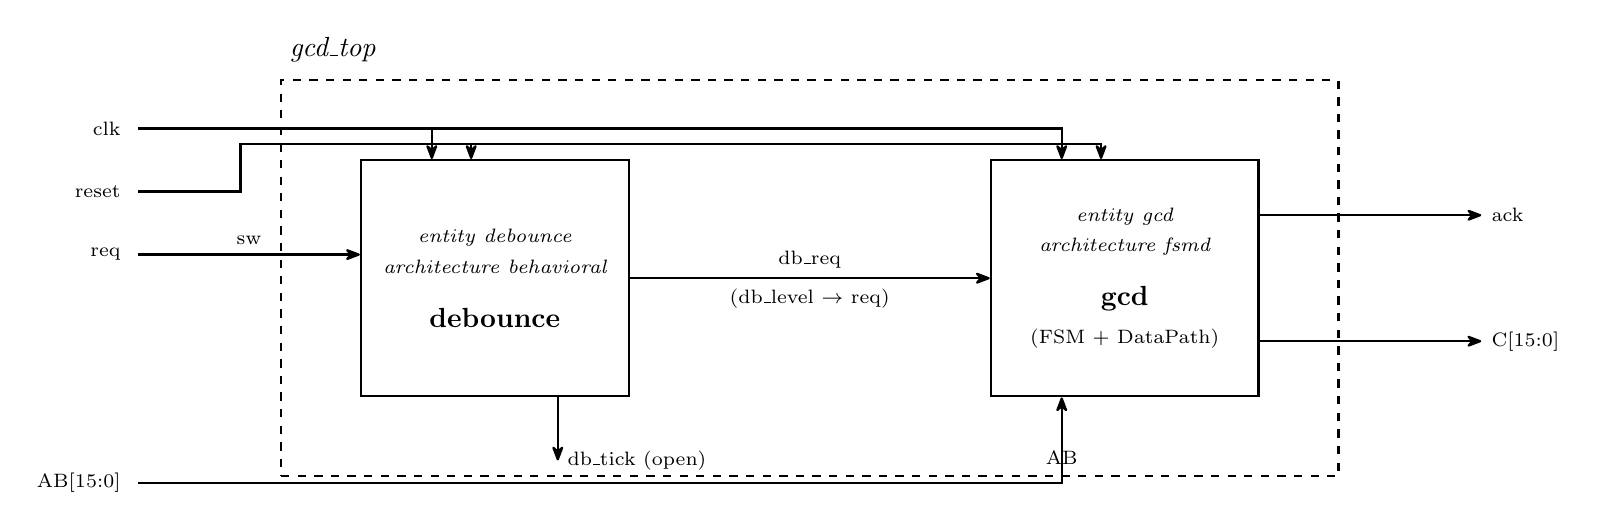
\begin{tikzpicture}[
  >={Stealth[round]},
  every edge/.style={draw, ->, thick},
  block/.style={draw, thick, minimum width=34mm, minimum height=30mm, align=center, font=\small},
  toplevel/.style={draw, thick, dashed, inner sep=10mm},
  portlabel/.style={font=\scriptsize},
]

  % ---------- inner blocks (entity / architecture shown inside, as a black box) ----------
  \node[block] (DEBOUNCE) at (0,0) {
    \scriptsize\itshape entity debounce \\
    \scriptsize\itshape architecture behavioral \\[3mm]
    \normalsize\upshape\textbf{debounce}
  };

  \node[block] (GCD) at (8,0) {
    \scriptsize\itshape entity gcd \\
    \scriptsize\itshape architecture fsmd \\[3mm]
    \normalsize\upshape\textbf{gcd} \\[1mm]
    \scriptsize\upshape (FSM + DataPath) 
  };

  % ---------- top-level boundary ----------
  \node[toplevel, fit=(DEBOUNCE)(GCD)] (TOP) {};
  \node[font=\itshape] at (TOP.north west) [anchor=south west, yshift=1mm] {gcd\_top};

  % ---------- top-level input ports ----------
  \coordinate (clk_in)   at ($(TOP.west)+(-1.8,1.9)$);
  \coordinate (reset_in) at ($(TOP.west)+(-1.8,1.1)$);
  \coordinate (req_in)   at ($(TOP.west)+(-1.8,0.3)$);
  \coordinate (AB_in)    at ($(TOP.west)+(-1.8,-2.6)$);

  \node[portlabel, left=1mm of clk_in]   {clk};
  \node[portlabel, left=1mm of reset_in] {reset};
  \node[portlabel, left=1mm of req_in]   {req};
  \node[portlabel, left=1mm of AB_in]    {AB[15:0]};

  % clk, reset fan out to both blocks (enter above the block text, clear of it)
  \draw[->, thick] (clk_in)   -| ($(DEBOUNCE.north)+(-0.8,0)$);
  \draw[->, thick] (clk_in)   -| ($(GCD.north)+(-0.8,0)$);

  % reset: rise above the blocks first (like clk), then fan out, so it never
  % crosses through the block outlines on its way in
  \coordinate (reset_elbow) at ($(TOP.west)+(-0.5,1.7)$);
  \draw[->, thick] (reset_in) -| (reset_elbow) -| ($(DEBOUNCE.north)+(-0.3,0)$);
  \draw[->, thick] (reset_in) -| (reset_elbow) -| ($(GCD.north)+(-0.3,0)$);

  % req -> debounce.sw
  \draw[->, thick] (req_in) -- node[portlabel, above] {sw} (DEBOUNCE.west |- req_in);

  % AB -> gcd.AB, routed below both blocks, well clear of db_tick
  \coordinate (AB_gcd) at ($(GCD.south)+(-0.8,0)$);
  \draw[->, thick] (AB_in) -| node[portlabel, above, pos=0.55] {AB} (AB_gcd);

  % ---------- internal signal: debounce.db_level -> gcd.req ----------
  \draw[->, thick] (DEBOUNCE.east) -- node[portlabel, above] {db\_req} node[portlabel, below] {(db\_level $\to$ req)} (GCD.west);

  % db_tick left open (short stub below debounce, clear of the AB wire)
  \coordinate (dbtick) at ($(DEBOUNCE.south)+(0.8,-0.8)$);
  \draw[->, thick] (DEBOUNCE.south -| dbtick) -- (dbtick);
  \node[portlabel, right] at (dbtick) {db\_tick (open)};

  % ---------- top-level output ports ----------
  \coordinate (ack_out) at ($(TOP.east)+(1.8,0.8)$);
  \coordinate (C_out)   at ($(TOP.east)+(1.8,-0.8)$);

  \draw[->, thick] (GCD.east |- ack_out) -- (ack_out) node[portlabel, right] {ack};
  \draw[->, thick] (GCD.east |- C_out)   -- (C_out)   node[portlabel, right] {C[15:0]};

\end{tikzpicture}
\end{document}
